\documentclass[a4paper,11pt]{article}
\usepackage[utf8]{inputenc}
\usepackage[margin=2.5cm]{geometry}
\usepackage{times}
\usepackage[compact]{titlesec} 
%%%% Compress space on the page
\titlespacing{\section}{0pt}{0pt}{0pt}
\AtBeginDocument{%
  \setlength\abovedisplayskip{0pt}
  \setlength\belowdisplayskip{0pt}}
\usepackage{sectsty}
%%%% Make all section headings sans serif
	\allsectionsfont{\sffamily}
\usepackage{fancyhdr}
\usepackage{amsmath,amssymb,amsfonts}
\usepackage{algorithmic}
\usepackage{graphicx}
\usepackage{textcomp}
\usepackage{xcolor}
\usepackage{array,etoolbox,multirow}
\usepackage{float}
\usepackage{caption} 
%%%% Make captions align to the left and italic
\captionsetup{justification=raggedright,singlelinecheck=false,font=it}
\usepackage{multirow}
\captionsetup[table]{skip=6pt}
\usepackage{natbib}
%%%% Make Harvard citations use an easier format
\let\cite\citep
%%%% for in-text citations, use \citet{...}

%%%% Changing headers and footer for ECIS conference requirements
\pagestyle{fancy}
\fancyhf{}
\renewcommand{\headrulewidth}{0pt}
\fancyhead[LO,LE]{\textit{\fancyplain{} Enabling BD through distributed-domain-driven RA}}
\lfoot{\textit{\fancyplain{} Thirtieth European Conference on Information Systems (ECIS 2022), Timișoara, Romania}}
\rfoot{\textit{\fancyplain{} \thepage}}

%%%% Changing the abstract format for ECIS conference requirements
\renewenvironment{abstract}
  {\quotation
  {\bfseries\noindent{\large\sffamily\abstractname}\par\nobreak\smallskip}    \noindent\itshape}
  {\endquotation}
\renewenvironment{quotation}{%
  \list{}{%
    \leftmargin0cm
    \rightmargin\leftmargin
  }
  \item\relax
}
{\endlist}

\newcommand{\hc}{[\textit{citation hidden}]\textnormal{}}

\title{Towards a domain-driven distributed reference architecture for big data systems}
\date{}

%\author{ \begin{tabular}{ll}Pouya Ataei & Alan Litchfield \\
%Auckland University of Technology & Auckland University of Technology \end{tabular}}



\begin{document}
\maketitle{}
	 
\begin{abstract}
 Issues spurred by changes in development approaches that shorten product delivery cycles, the adoption of digital devices and services, and the deployment of decentralised infrastructure increase the rate of generation of data. The accelerated growth of data could be called the era of big data and forced a paradigm shift in data engineering because the variety, velocity and volume of data overwhelmed existing systems. While companies attempt to extract benefit from big data, success rates are still low. Challenges such as rapid changes in technology, organizational culture, complexity in data engineering, impediments to system development, and a lack of effective big data architectures mean that only an estimated 20\%{} of companies achieved their goals. To this end, this study explores a domain-driven distributed big data reference architecture that addresses issues in data architecture, data engineering, and system development. This reference architecture is empirically grounded and evaluated through deployment in a real-world scenario as an instantiated prototype, solving a problem in practice. The results of the evaluation demonstrate utility and applicability but with architectural trade-offs and challenges.
\end{abstract}


\noindent{}\emph{Keywords: Big data, Reference architecture, Big data architecture, Domain-driven architecture, Distributed architecture}


\section{Introduction}
\nobreak{}
The ubiquity of digital devices and software applications allow users to generate data at an unprecedented rate. Almost all aspects of human life is integrated with some sort of software system that is performing computational processes on data. The rapid expansion and evolution of data from a structured element that is passively stored in the database to something that is used to support proactive decision making for business
competitive advantage, have dawned a new era, the era of Big Data (BD). The BD era emerged when the velocity, variety, and volume of data overwhelmed existing system capability and capacity to effectively and efficiently process and store data 
%\cite{AtaeiApsec,AtaeiACIS}.
\hc{}. 

BD is the practice of crunching large sets of heterogenous data to discover patterns and insights for business competitive advantage 
%\cite{rada2017hype}.
\hc{}.
 Since the inception of the term, ideas have ebbed and flowed along with the rapid advancements of technology, and many strived to harness the power of BD. Nevertheless, there are many failed attempts, for example, as of 2021 only 13\%{} of organizations succeeded in delivering on their data strategy \cite{DataBricksSurvey} and 20--24\%{} successfully adopted BD \cite{NewVantageSurvey,GartnerSury}. Among the challenges of adopting BD, latent complexity in data engineering, rapid technology changes, data architecture and a poor supply of skilled data engineers are highlighted. 
%\cite{rad2017big}.
\hc{}.  

A BD system is motivated by an array of functional requirements and quality goals. But if this system is to be successful, it must achieve these functional requirements within an acceptable performance, availability, modifiability and cost parameters. The software architecture is the key ingredient in determining whether these goals are attainable, before colossal amount of resources are committed to it. The initial design, development and deployment of a BD system does not mean success. As system grows larger, data providers and data consumers increase, data variety expands, data velocity extends, and metadata becomes increasingly more challenging to handle. This means, only a handful of highly specialized data engineers would be able to understand the system internals, resulting in silos, burnt out and potential friction.

This creates a perfect ground for immature architectural decisions that result in fragile systems that are difficult to maintain and scale. To this end, we explore the concept of generally applicable domain-driven distributed software Reference Architecture (RA) that is technology independent. The contribution of our work is threefold: 1) design theories that critique current BD RAs, 2) design theories that creates the foundation of our RA, 3) the artifact. 


\section{Background}
In this section, the current state of BD architectures, identification of the study focus, and study objectives are provided. Two important elements are discussed, the current state of BD architectures and why RA is needed.

\subsection{Overview of BD architectures}
In this overview, three generations of BD architecture are presented. A key issue observed in all the approaches analyzed was the existence of an architecture featuring a federated or contiguous data pipeline to  channel all data without any consideration for data quality and ownership. Thus, data that logically belongs to different domains are aggregated and processed together, creating impediments to scalability and maintainability. In addition, cross-cutting concerns such as metadata management, security, privacy, data ownership and interoperability are hardly addressed.

\begin{description}
    \item[Enterprise Data Warehouse] Generally built around a monolithic data warehouse, Extract-Transform-Load (ETL) processes, and data analysis and visualization/presentation software. Enterprise Data Warehouses are typically designed against specific requirements that limits how BD characteristics may be exploited effectively. As the Enterprise Data Warehouse expands and data consumers and data providers increase, ETL processes become increasingly difficult to maintain and manage. This results in slower transaction processing and increased dependency on a small group of specialized staff. Such dependency creates silos that creates friction within and between teams and organizational boundaries. Furthermore, this monolithic architecture makes scaling, maintenance, and the extension of data engineering pipelines (for example, the addition of new transformations or data structures)  difficult and time consuming and thus, expensive. Systems developed underlying this class of architecture usually fail to effectively handle the requirements of a modern BD analytics.
    \item[Data Lake] To address general issues in data warehousing, a new BD ecosystem emerged as the Data Lake. In this approach, there isn't much data transformation before data are written into the Data Lake and data are usually retrieved from data scientists and machine learning engineers in raw format. While Data Lake architectures address some issues with data warehouse architectures, such as the capability of handling data variety, optimization features may be lacking. For example, if the number of data consumers and providers increase, the data stored in data lake increases, and without any clear data domains, this will soon turn into a data swamp. Furthermore, data quality decreases over time firstly because no data owners are linked to stored data, and secondly because the BD stack is managed by specialized data engineers that may become siloed with ever-increasing backlogs. Data engineers may have little awareness of the semantics and value of the data they are processing, how data are useful to the business, and which domain data belongs to. Consequently, data quality reduces making maintenance and scaling a daunting task. 
    \item[Cloud Based Solutions] Considering the sheer cost of running a data engineering cluster on-premise, the current talent gap faced in the market, and complexity of provisioning the infrastructure of ever-increasing data processing loads 
    %\cite{rada2017hype},
    \hc{},
     companies may choose to deploy on the Cloud for their BD solutions. The current technological generation leans towards architectures that provide Lambda or Kappa for stream processing or batch processing, or frameworks that unify the two like Databricks or Apache Beam. Whereas this generation of BD architectures might bring reduced cost and complexity for data architects, it still suffers from the same architectural challenges of having no clearly defined data domains, siloed specialized data engineers, and a monolithic pipeline BD architecture.
\end{description}

To address these issues, we explore a domain-driven distributed RA for BD systems and propose an RA that addresses some of the challenges. The RA is inspired by the advances in software engineering architectures such as microservices, and reactive systems. Moreover, this RA is inspired by the concept of data mesh \citep{dataMeshBook} and domain-driven design \citep{evans2004domain}.


\subsection{Why a Reference Architecture?}
Software architecture is an artefact that aims to satisfy business objectives through a software solution that is adaptable, cost-efficient, maintainable, and scalable. In addition, it allows for the capture of design issues at an early stage in the development process. Whereas this practice can be applied to any class of system, it is particularly useful in the design and development of complex system such as BD 
%\cite{AtaeiApsec}.
\hc{}
 Despite the known complexity of BD systems, the development, analysis, and design of an RA that incorporates best practices, techniques, and patterns and that supports the achievement of BD goals is possible \cite{ataei2022state}. Therefore engineers and architects can better absorb the complexity of BD system development and make it tractable. This can be seen in Software Product Line (SPL) development where RAs that provide generic artefacts can be instantiated and configured for use in specific system domains \cite{Derras,Cloutier}.


Furthermore, RAs are used to standardize an emerging domain, \citet{Iso18384-1}, and in diverse environments like NASA space data systems \cite{NASA}.Therefore, RAs are effective for addressing complex BD system development, because: 1) RAs promote adherence to best practice, patterns, and standards, 2) RAs can endow the architecture team with increased openness and interoperability, incorporating architectural patterns that provide desirable quality attributes, and 3) RAs serve as the locus of communication, bringing various stakeholders together. 

\section{Related Work}

The application of RAs for solving challenges in data architecture is not a new concept and the production of BD RAs has had support from governmental agencies, for example the NIST BD RA (NBDRA) \cite{Chang}, and from industry, for example IBM \cite{quintero2019ibm}, Microsoft \cite{levin2013big}, Oracle \cite{cackett2013information}, SAP \cite{SAPRA}, and ISO \cite{ISO20547}. In addition, Lambda \cite{kiran2015lambda} and Kappa \cite{lin2017lambda} provide BD architectures at the level of an RA. In addition, conceptual RAs have been proposed \cite{Maier,suthakar2017scalable,framework2015draft}.

Numerous domain specific RAs have been developed, for example, in national security \cite{Klein}, and Internet of Things (IOT)  \cite{weyrich2015reference}. Some effort has been put into the adoption of microservices architecture for BD systems such as Neomycelia 
%\cite{AtaeiApsec}
\hc{}\hspace{1mm}
 and Phi \cite{maamouri2021phi}. 
 
The RAs investigated may be instantiated but outwardly, most appear to be conceptual studies and do not provide sufficient data on cross-cutting concerns such as data quality, data integrity, data ownership, security, and privacy. Therefore, by providing a domain-driven distributed architecture for BD systems, this study extends current learnings by addressing the current limitations of BD RAs. 
The RA presented here focuses on the logical separation of data into domains through event-driven communication and with clearly defined boundaries %\citet{AtaeiApsec}.
\hc{}. 

\section{Method}
The study is comprised of two phases: the first is the identification of high level requirements of the artefact, and second applies a well-established methodology for building the RA. These phases are elaboroated in the following sub-sections.


\subsection{Requirement Specification}
Prior to RA modelling and design, the desired properties of the artefact are defined as requirements. System and software requirements range from a sketch on a napkin to formal (mathematical) specifications. Therefore, the kind of requirements for the purpose of this study are defined in an exploration of the body of evidence. 
%\cite{AtaeiACIS}.  
\hc.
% An analysis of existing RAs developed for BD systems offers general requirements, the spectrum of BD RAs, and how they are designed 


Defining and classifying software and system requirements is a common subject of debate. \citet{sommerville2011software} classify requirements as three levels of abstraction; user requirements, system requirements, and design specifications. These are mapped against user acceptance testing, integration testing, and unit testing. In this study, a more general framework provided by \citet{laplante2017requirements} is adopted. The adopted approach provides three categories as functional, non-functional, and domain requirements. The objective in this phase is to define the high-level requirements of BD systems, thus non-functional requirements are not fully explored. 


After clarifying the type of requirements, we assessed current BD RAs and their requirements to better understand the domain. We realized a common approach to classifying requirements is through BD characteristics such as Velocity, Veracity, Volume, Variety and Value \cite{ataei2022state}.
%\cite{Bahrami2015,rad2017big,Chen2016a}.
\hc{}\cite{Bahrami2015,Chen2016a}.
 In an extensive effort, NIST Big Data Public Working Group embarked on a large scale study to extract requirements from variety of application domains such as Healthcare, Life Sciences, Commercial, Energy, Government, and Defense \cite{Chang}. The result of this study was the formation of general requirements under seven categories. \citet{volk2020identifying} categorizes nine use cases of BD projects sourced from published literature with a hierarchical clustering algorithm. Bashari et al. 
%\cite{bashari2016security}
\hc{}
 focus on security and privacy requirements for BD systems, \citet{yu2019components} present modern components of BD systems , using goal oriented approaches, \citet{eridaputra2014modeling} create a generic model for BD requirements, and  \citet{al2016characteristics} investigate general requirements to support BD software development. 



By analyzing these studies and by evaluating the design and requirement engineering required for BD RAs, a set of high-level requirements based on BD characteristics is established. A rigorous approach to present software and system requirements that offers informal methods of model verification is identified because such methods are well established in the industry and academia \cite{kassab2014state}.  Our approach for representing functional requirements follows the guidelines in \emph{ISO/IEC/IEEE standard 29148} \cite{ISO29148}. The requirements representation is organized in system modes, where the major components of the system and then the requirements are described. This approach is inspired by the requirement specification expressed for NASA Wide-field InfraRed Explorer (WIRE) system \cite{laplante2017requirements} and the Software Engineering Body of Knowledge (SEBoK) \cite{abran2004software}.

The requirements are categorized by the major characteristics of BD (Table~\ref{table-requirements}); value, variety, velocity, veracity, volume %\cite{rada2017hype}
\hc{},
 and security and privacy 
%\cite{bashari2016security}. 
\hc{}.


    \begin{table}[h!t]
    \centering
    \renewcommand*{\arraystretch}{1.8}
    \begin{tabular}{|l|p{12cm}|}
	\hline
	\textbf{Category} & \textbf{Requirements} \\
        \hline

        Volume &

        \textbf{Vol-1)} System shall support asynchronous, streaming, and batch processing to collect data from centralized, distributed, and other sources, \textbf{Vol-2)} System shall provide scalable storage. 
        \\
        \hline
        Velocity & 
        
        \textbf{Vel-1)} System shall support variable intensity of data transmission between data sources, \textbf{Vel-2)} System needs to stream data to data consumers in a timely manner, \textbf{Vel-3)} System shall provide the capability to ingest multiple, continuous, time varying data streams, \textbf{Vel-4)} System shall support fast search from streaming and processed data with high accuracy and relevancy, \textbf{Vel-5)} System may provide the capability to process data in real-time or near real-time. 
        \\ 

        \hline

        Variety & 

        \textbf{Var-1)} System shall support data in various formats ranging from structured to semi-structured and unstructured data, \textbf{Var-2)} System shall support aggregation, standardization, and normalization of data from disparate sources, \textbf{Var-3)} System shall support adaptations mechanisms for schema evolution, \textbf{Var-4)} System may provide mechanisms to automatically include new data sources 
        \\

        \hline

        Value & 
        
        \textbf{Val-1)} Shall provide capability to handle compute-intensive analytics and machine learning processes, \textbf{Val-2)} System shall provide support for batch and stream processing, \textbf{Val-3)} System shall support different output file formats for different purposes, \textbf{Val-4)} System shall provide support for streaming of results to consumers.
        \\

        \hline

        Security \& Privacy & 
        
        \textbf{SaP-1)} System shall provide protection and retention of privacy and security measures for sensitive data, \textbf{SaP-2)} System shall provide protection of data and processing nodes via access control methods and policy-driven authentication at multiple levels. 
        \\

        \hline
        
        Veracity &
        
        \textbf{Ver-1)} System shall support data quality curation including classification, pre-processing, format, reduction, and  transformation, \textbf{Ver-2)} System shall support data provenance including data life cycle management and long-term preservation.
        \\
        \hline
  
    \end{tabular}
        \caption{BD system requirements}\label{table-requirements}
    \end{table}



\subsection{Artefact Development Method}
There are several approaches to the systematic development of RAs. \citet{Cloutier} demonstrate a high-level model for the development of RAs through the collection of contemporary architectural patterns and advancements. Bayer et al \cite{bayer1999pulse} introduce a method for the creation of RAs for product line development called PuLSE DSSA. \citet{stricker2010creating} present the idea of pattern-based RA for service-based systems and use patterns as first class citizens. Similarly, \citet{nakagawa2014consolidating} present a four-step approach to the design and development of RAs. Influenced by ISO/IEC 26550 \cite{wg2015iso}, \citet{Derras} present a four-phase approach for practical RA development in the context of domain engineering and SPL.


Additionally, \citet{galster2011empirically} propose a 6-step methodology with two primary concepts: empirical foundation and empirical validity. Taking all these into consideration, an empirically-grounded RA methodology provides the most appropriate methodology to meet the purposes of this study. Reasons being that this methodology for RA development is adopted more than any other, and that the methodology supports the objectives of this study. 

Nevertheless, the methodology needed to be augmented with other approaches to arrive at the desired level of rigour and relevance.  For example, comprehensive guidelines on how to collect empirical data in step 3 and how to model the data collected.  \citet{Nakagawa} provided
investigation guidelines and the RAModel concept. Also, the methodology does not describe how to evaluate the RA, thus, a more systematic and stronger evaluation approach is required. To address this, an instantiation the RA is deployed in a real world practice, then the Architecture Tradeoff Analysis Method (ATAM) \cite{KazmanATAM} is applied to evaluate the artefact. The methodology constitutes six steps as below:  


\begin{description}
\item[1. Decision on type of RA] Prior to the development of the RA, the type needs to be identified that will determine the structure, data to be collected, and objectives. A classification framework and the results of an Systematic Literature Review (SLR) are applied \cite[\hc{}]{angelov2009classification}.
%\cite{angelov2009classification,AtaeiACIS}.
 

In this classification framework, RAs are categorized as standardization RAs and facilitation RAs. The domain-driven distributed RA chosen for the purposes of this study addresses two essential goals: 1) openness and interoperability between heterogenous components of a BD ecosystem and 2) facilitation of BD system development and data engineering. Accordingly, the output artefact is classified as `classical standardization RA designed to be implemented in multiple organizations'. 

\item[2. Selection of Design Strategy] According to \citet{galster2011empirically}, RAs can have two major design strategies to them; 1) RAs that are based on existing patterns, principles and architectures, and 2) RAs that are developed from scratch. Designing RAs from scratch is scarce and usually happens in areas that have received no attention (could be BD in 2004). On the other hand, RAs are proven more successful when built from the proven practices \cite{Cloutier}. 

The RA developed for the purposes of this study is a research-based RA based on existing RAs, concrete architectures, patterns, standards and best practices.

\item[3. Empirical Acquisition of Data] Due to limitations witnessed by the \citet{galster2011empirically} methodology, we have augmented this phase to increase transparency and systematicity, by employing a SLR for data collection. 

This phase is comprising of three major undertakings; 1) identification of data sources, 2) capturing data from the selected sources and 3) synthesis of the selected data. 

\emph{Identification of Data Sources:} For this sub-phase, we employed the ProSA-RA's `information sources investigation'. To unearth the essential architectural quanta, we selected our sources as `publications'. In order to capture the essence of existing body of knowledge from publications, we conducted a SLR. This SLR is an extension of 
%\citet{AtaeiACIS}.
\hc{}.
 The methodology as described in 
 %\citet{AtaeiACIS}
 \hc{}
 was followed but this time for the years 2021 and 2022. The main objective of this SLR is to find common architectural constructs among existing BD architectures, and highlight limitations.



\emph{Capturing data from the selected sources:} After having pooled quality literature, the study embarked in the process of capturing data. We used to software Nvivo for coding, labelling and classifying studies. 

\emph{Synthesizing Data:} Codes highlighted patterns and patterns resulted in themes, which grounded the design theories necessary to build this RA. Our aim was to capture the body of knowledge and project it into our RA. 

\item[4. Construction of the RA] The requirements, themes, patterns and theories previously identified inform the design and development.  RA components are defined and how they ought to be integrated, how they should communicate, how do they address the requirements and what are the architectural tradeoffs.  \citet{ISO42010} provided the structure and it was modeled with Archimate and the Architecture Description Language (ADL) in ISO/IEC/IEEE 42010.

\item[5. Enabling RA with variability] One of integral elements that help with instantiation of the RA is variability. This enables RA to remain useful as a priori artefact when it comes down to organization-specific regulations, and regional policies that may constrain the architect's freedom in design decisions. For the purposes of this study, we chose to represent variability by the means of ``annotation'' as recommended as on of the three accepted approaches by \citet{galster2011empirically}.


\item[6. Evaluation of the RA] This last phase of the methodology is to ensure that RA has achieved its goal, and to test its effectiveness and usability. Based on \citet{galster2011empirically}, the quality of the RA can be assessed through its utility, correctness, and how efficiently it can be adopted and instantiated. However, while established methods for assessing concrete architectures exist, most are not applicable to RAs \cite{Avgeriou}. 

This is due to the inherent properties of RAs such as level of abstraction, and lack of clearly defined group of stakeholders. Various authors have attempted to solve this issue; for instance, \citet{angelov2008towards} has attempted to adapt ATAM for use with RAs. Thus in applying ATAM, we have instantiated the RA and then evaluated the prototype in practice. 
\end{description}


\section{Domain-driven Distributed RA for BD Systems}
\nobreak{}
The principles upon which the RA is built requires that it is 1) Domain-driven: to address data quality, siloed teams, data swamp issues and communication issues, affecting velocity, variety, and veracity requirements; 2) Distributed: to address the challenges of scaling monolithic data systems affecting velocity, and volume requirements; 3) Data as a service: to allow for increased discoverability of data and autonomy of various analysis and data science teams without frictions with data engineers affecting value, variety, veracity, security and privacy requirements; 4) Governance through a federated service: the prevent team-based and rather immature decisions that may not be in-line with global organizational visions, policies, standards and procedures, affecting all requirements; 5) Event driven: to address point-to-point communication issues that arises in distributed systems, affecting velocity requirement. Additionally, the elements of the RA that are annotated with the phrase `variable' can be modified, adjusted or even omitted based on the architect's decision. 


\begin{figure}[h!t]
    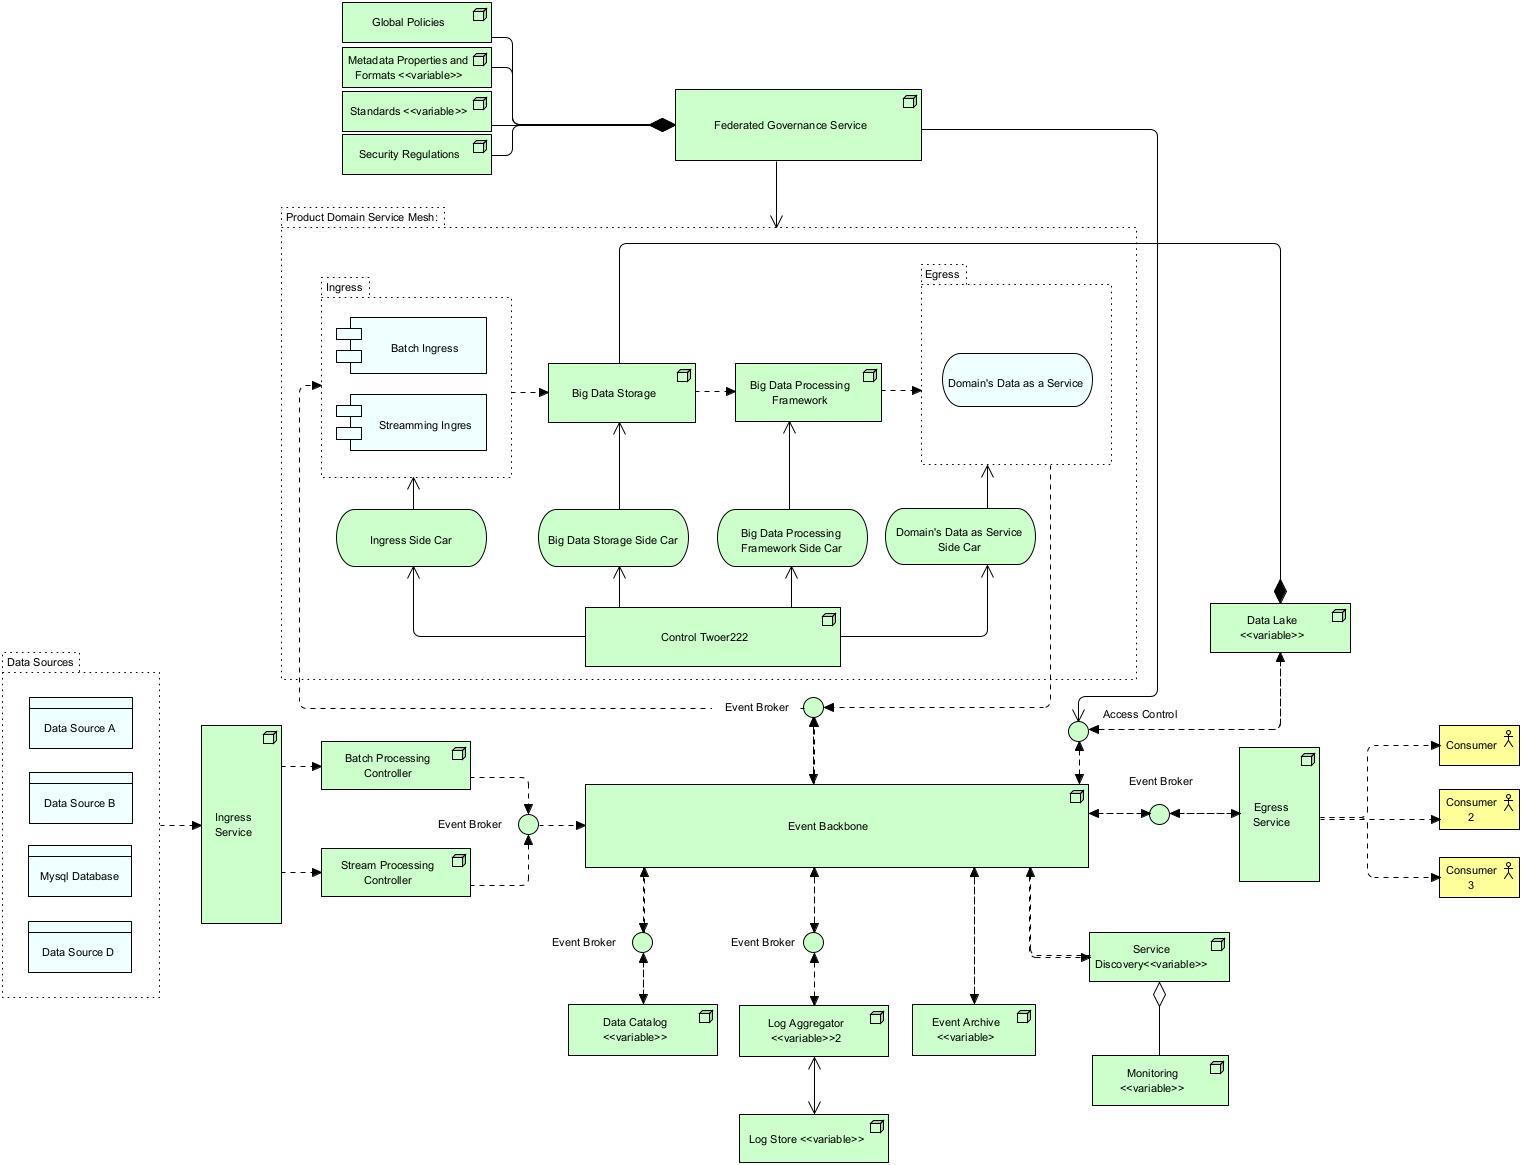
\includegraphics[width=\linewidth]{media/Metamycelium.jpg}
    \caption{domain-driven Distributed RA}
    \label{fig-RA}
\end{figure}

To produce the RA (Figure~\ref{fig-RA}), design iterations have been inspired by microservices architectural patterns \cite{richardson2018microservices}. To shift from collecting data in monolithic data lakes and data warehouses to converging data through a decentalized and distributed mesh of data products communicating through standard interfaces, the RA shall be domain-driven and distributed. This addresses the limitations in current BD architectures. This RA comprises 11 principal and 9 variable components, discussed below:

\begin{description}
    \item[Ingress Service] This service is responsible for controlling traffic into the system. Depending on the type of request, this service will load balance either into a batch processing controller or a stream processing controller. Ingress is an asynchronous load balancer designed to eliminate choke points, handle SSL termination, and provide with extra features such as named-based virtual hosting. This component addresses the requirements Vol-1, Vol-2, Var-1, Var-3, Var-4, Val-1, Val-3, Val-4, SaP-1 and SaP-2. 
    
    \item[Batch Processing Controller] This controller is responsible for handling batch processes. That is, it is responsible for receiving request for batch processing, and communicating it to the event broker. Due to the batch nature of the requests, the controller can decide to achieve this in a bulk and asynchronous manner. This component addresses the requirements Vel-1, Val-1, and Val-2. 
    
    \item[Stream Processing Controller] This controller achieves similar thing to the batch one, with a difference that it has to handle a different nature of requests. Stream events are synchronous in nature and require hight through-put. Having a specific service for stream processing requirements promote tailored customization that best suit the varying nature of stream events. This component addresses the requirements Vol-1, Vel-1, Vel-2, Vel-4, Vel-5, Val-2,  
    
    \item[Event Broker] An important architectural construct designed to achieve inversion of control. As the system grows, more nodes and services are added, communication channels increase, and there is a need fore new events to be dispatched. As each service communicates through the event backbone, each service will be required to implement its own event handling module. This can easily turn into a spaghetti of incompatible implementations by different teams, and can even result in unexpected behaviors. To address this issue, an event broker is introduced to each service which has one main responsibility; communication with event backbone. This component indirectly addresses the requirements Val-1, and Ver-1.  
    
    \item[Event Backbone] Event backbone is the heartbeat of the system, facilitating communication between all services. Where as this service is displayed as one technology service in the Archimate diagram, we recommend the event backbone to be designed underlying distributed paradigms itself. This is to ensure scalability as the number of topics and events grows. Event backbone and its relationship to other nodes is analogous to a dance troupe in which dancers move to the rhythm relative to their position. In this case, the event backbone is the music and services are the dancers. Thus, services are only responsible for dispatching events in a `dispatch and forget' model, subscribing to topics they are interested. This component addresses the requirements Vel-1, Vel-2, Vel-3, Vel-4, Vel-5, Val-1, Val-2, Ver-1, Ver-2, and Ver-3.
    
    \item[Egress Service] This services is responsible for providing necessary APIs to the consumers of the system, third parties or other BD systems. This allows for the openness of the architecture, and lets data scientist and business analyst easily request the data necessary for their work-loads. This also promotes the idea of self-serve-data through service discovery, data catalogue and product domains. This component can also be tuned for QoS networking, and other low computational functions if needs be. This component addresses the requirements Vel-2, Vel-4, Val-3, Val-4, SaP-1, and SaP-2. 
    
    \item[Product Domain Service Mesh] Driven by the idea of domain-driven design, every product has it is own bounded context and ubiquitous language, and is technically governed by a service mesh. Every service mesh is made up of a batch ingress, stream ingress, BD storage, BD processing framework, domain's data service, together with the control tower and the side cars. These components provides the necessary means for the domain to achieve its ends in regards to BD processing. This is to enable high cohesiveness, low coupling and clear interfaces among services. This component indirectly addresses Vol-1, Vel-3, Vel-4, Vel-5, Var-1, Var-2, Var-3, Val-1, Val-2, Val-3, Val-4, Sap-1, SaP-2, Ver-1, Ver-2, and Ver-3.
    
    \item[Federated Governance Service] Given the distributed nature of the architecture and sheer number of moving parts with varying life-cycles; there is a need for some global contextual standards and policies that are designed to streamline processes and avoid losses. This is not to limit the autonomy of teams, but to inject them with best practices and organizational policies that tend to reflect the capability framework, regional limitations, and legal matters that can cause sever damage to the business. This component can indirectly affect all requirements.
    
    \item[Data catalog] As data products increase in the system, more data become available, interoperability increases, and thus services have to know who provides what data. Data catalog is responsible for keeping a catalog of all data available among services with relative paths to fetch those data. This component addresses the requirements Vel-4, Var-1, Var-3, and Var-4.

    \item[Log Aggregator and Log Store] Operating underlying a distributed paradigms, requires a shift in a way that logging occurs. This means system cannot rely only one applications reporting logs in a single environment, but there's a need for a distributed tracing that shows a lifecycle of a process and how it went through different services. Therefore this RA benefits from the popular log aggregator pattern initially released by the microservices community, to allow fo graceful scaling of system's logging strategy. This component indirectly addresses the requirements Vol-1, Vel-1, Val-1, and Ver-1. 
    
    \item[Event Archive] One of the main challenges of this architecture is it is reliance on event backbone. Whereas event backbone itself is recommended to be distributed and fault tolerant, event archive further solidifies the service recovery from unexpected events. This implies that, if the event backbone went out of service, the history of events can be stored and retrieved from the event archive to bring various services to the current state of operation. This component indirectly addresses the requirements Vol-1, Vel-1, Val-1, and Ver-1. 

    \item[Data Lake] Whereas product domains are demarcated and boundaries are well-defined, we do not find it necessary for each domain to maintain it is own data lake. This is under the assumption that a lot of data are now processed at the time of storage, and is required whenever there is a analytical business case for it. Whereas there isn't a data lake per domain, different domains can have a quota in the data lake that is owned and handled by access control. This component addresses the requirements Vol-2, Vel-1, Var-1, Var-3, Var-4, Val-3.
    
    \item[Service Discovery] In a distributed environment, services need to find each other in order to communicate their means. Service discovery solves this issue with primary responsibility of identifying services and answering queries about services. This is achieved by services registering themselves to service discovery on boot up. This component indirectly addresses the requirements Vel-2, Vel-4, Var-2, Var-4, Val-3, Val-4, SaP-2. 

    \item[Monitoring] To take proactive measures for the overall health of the system and its considerable moving parts, one needs to actively monitor the state of the individual nodes and the overall flow of things. Services emit large amounts of multi dimensional telemetry data that can be read and analyzed for the supporting actions. Monitoring services help storing these data to fuel proactive actions. This component indirectly addresses all requirements. 

\end{description}


\section{Evaluation}

The aim of the evaluation is to assess the application and utility of the RA as a context-specific concrete architecture that solves an actual problem. For this purpose ATAM has been chosen because of it's pedigree both in academia and industry, and has been applied to variety of architectures and scales \cite{SoftwareArchitectureKazman}. While the evaluation could have been achieved with technical action research,  ATAM aligns with the conceptual architectural constructs and provides rigor \cite{wieringa2014design}. 

The application of ATAM uncovered key architectural tradeoffs, risks, and sensitivity points, which provided confidence in the RA. While ATAM is normally conducted by an outside team after the architecture is created, ATAM was tailored to the requirements of our study. A prototype from the RA was created and then the ATAM steps were taken in the evaluation. For the instantiation of the RA, ISO/IEC 25000 Software Product Quality Requirements and Evaluation (SQuaRE ) \cite{ISO25000} was used for technology selection. 

% We found mature technologies that could support our requirements, and opted not to develop any tools from scratch for the purposes of this study. It is also worth mentioning that, 

Node JS for all APIs was chosen and custom scripting, with Nginx for ingress, AWS Lambdas for stream and batch processing controllers, Kafka for event backbone, Kafka event brokers as the event broker, AWS application load balancer as the egress load balancer, Istio as the control tower, Envoy as the side car, Kubernetes as the container orchestrator, AWS S3 as the BD store and event archive, and Data Bricks for stream and batch processing. The aim was to incorporate most components of the RA into this instance, however logging, monitoring, service discovery, federated governance service, and data catalog are omitted. 

We dot not describe the ATAM steps in detail, but explain the evaluation process instead. To ensure security and intellectual property of the practice, some evaluation detail is omitted but that does not affect the integrity of the evaluation.  

\subsection{Phase 1}
\nobreak{}
Evaluation was performed in a subsidiary of a large scale international company that specializes in practice management software for veterinary professionals. The company provides services to hospitals via Software as a Service (SaaS) across the globe including some of the largest equine hospitals and universities. The company has several ambitions that include BD management and AI. 

The ATAM first step is the identification of relevant stakeholders. To ensure that we have not missed anything major in our design, the focus was on key stakeholders such as lead architects. Stakeholders that do not directly correlate with the prototype, such as the UI/UX designer, were not included. As a result, two lead development architects were invited; the head of product as a product owner responsible for the product in which the artefact is tested, and a quality assurance engineer and several developers. 

Step 1 provided the initial meeting in which ATAM was presented and a description of its purposes. In step 2, stakeholders discussed the background of the business and some of the challenges faced, and the current state of affairs, the primary business goals, and architecturally significant requirements. In step 3, the prototype was presented, with assumptions and variability points. 

Then architectural styles to achieve quality attributes were agreed upon. For availability, Kafka's partitions, Nginx worker connections, Data Lake and Istio were identified.  For performance, Nginx asynchronous processing, Kafka topics and consumers, AWS application load balancer, and Kubernetes deployments identified. For modifiability, the concept of domain-driven design, side cars, and event brokers were discussed. The approaches were then analyzed for tradeoffs, sensitivity points, and potential risks. 

In order to generate a utility tree, consensus on the most important quality attributes for the evaluation was required. Assumptions were presented and after discussion, taking into account concerns over privacy, agreement was reached that availability, performance, and maintainability were chosen. The utility tree was then created with the requirements: 1) performance: the system should be able to process real time streams under 1200 ms, queries from a data scientist should not take more than 2 hours 2) availability: the load balancer and data bricks cluster shall be have 99.999\% availability, and 3) modifiability: the new product domain should delivered within a month and with less than 5 persons.

Due to resource constraints, we skipped a preliminary analysis of architectural approaches in phase 1 and only conducted it after the scenarios had been prioritized. This did not negatively affect the evaluation process.



\subsection{Phase 2}
\nobreak{}
Scenarios are the quanta of ATAM and help capture architectural stimuli. Thus for this step, stakeholders were asked to prioritize three classes of scenario, growth, use-case, and exploratory scenarios. From this, 20 scenarios were pooled that stakeholders to voted on. The voting process yielded 5 scenarios, described as two user journeys: 1) The pet owner brings the pet to the veterinary hospital, the pet is diagnosed with cancer wherein the pet's environmental factors should be studied for potential clues for the root cause of cancer; 2) a pet owner brings the pet to the veterinary hospital, the cat's symptoms should be processed for early detection of Lyme disease. 

After identifying architectural approaches and prioritizing scenarios, we ran the scenarios against our prototype. This provides opportunity for heuristic qualitative analysis and identification of sensitivity points and tradeoffs. The process was initiated by creating a custom script to extract data from the company's mySQL database and send it through the ingress process. The topics for Kafka were created, then Nginx was configured to pass the requests to responsible lambdas for batch and stream processing. We then followed with event producers, Istio, Envoy, Kubernets, Data Bricks and the rest of the system. How architectural decisions contribute to the realization of each scenario was explained.

\subsection{Results}
\nobreak{}
While running the scenario simulations against, the architectural approaches were constantly assessed. Many implementation issues arose and sensitivity points noted. The true cost of the system, its trade offs, and potential challenges were realized. Based on these and stakeholder feedback, it was found that system quality, $Q_S$, is a function, $f$, of the quality attributes of performance, $Q_P$, availability, $Q_A$, and modifiability, $Q_M$, expressed as the equation $Q_S = f(Q_P, Q_A, Q_M)$.

For performance, cloud stress testing agent StressStimulus was applied. The stress test was run against the system and revealed that the cold start time (100-1000ms) of AWS Lambdas impact performance. However, for an accurate evaluation, we opted not to use micro-batch while using Data Bricks for stream processing. Also, to test the worst case scenario, the fair scheduling pool was not configured. 

Performance tests of the prototype included periodic data dispatch, large volume of data, and many concurrent requests. It became evident that latency, input/output, and object mutations negatively impacted performance. The event driven design produced better outcomes when handling simulations.  Therefore the system is sensitive to latency ($l$), side effects ($s$), and concurrency ($c$), expressed as $Q_P = h(l, s, c)$.

Next, the prototype was tested for availability. Since the system is distributed, a poorly handled failure in one service can create a ripple effect through other services. Through the implementation of circuit breakers in event brokers, the prototype can recover from this situation. To achieve a stable state, the prototype archives events in the event backbone before any failure. Moreover, health checks and alarms on pods in the Kubernetes cluster provide monitoring. 

Kubernetes ensures a minimum quantity of services are available through deployments and replica sets. The evaluation demonstrates that the architecture complies with 12 factor methodology and is deemed cloud native, which positively affected the availability score. Therefore, system availability is affected by the time it takes for circuit breakers to trip and become available again ($\mu_C$), failure of the event backbone ($\lambda_E$), and the time it takes for the services to recover ($\mu_S$), with $g$ being the fraction of time that the system is operating. Thus, system availability is expressed as $Q_A = g(\mu_C, \lambda_E, \mu_S)$.

Finally, the prototype was tested for modifiability. The distributed and domain-driven nature of the architecture made it easy to achieve the desired modifiability objectives. Adding a new data domain only required an extension of the HCL module, written in Terraform for the EKS cluster, and modify that with new Docker images. Brokers were also streamlined, so a new broker can be stood up within minutes. The certification lifecycle is handled by Istio, Local Cert Manager and Let's Encrypt. Therefore, system modifiability is sensitive to the provisioning, maintenance and configuration of Kafka ($K_a$), Kubernetes ($K_u$), and Databricks ($D$), and the skill set ($s$) required to achieve these. Thus, system modifiability is expressed as $Q_M = s(K_a, K_u, D)$. 

After analysis, two tradeoff points are identified: 1) Event brokers and the event backbone, and 2) service mesh. The event backbone was of concern and how it might turn into a bloated architectural component like ESBs in SOAs. However given the nature of the distributed system, the event archive, and event brokers, that is unlikely to be an issue because the event backbone is responsible for one function only, to provide communication between services. In addition, in the case of service outage, the order of events can be retrieved from the event archive and providing a stable state for the system. Event brokers facilitate modifiability by providing native event handling mechanisms but at a cost of one more layer and the potential latency that comes with it. Therefore, while providing positive impact on performance and maintainability, the event backbone can have negative impact on availability and reliability. Furthermore, event brokers provide positive impact on modifiability and availability without negatively affecting performance. 

The service mesh was a subject of concern. To get the service mesh operational required significant effort from developers. However, modifiability is positively affected longitudinally and the service mesh promotes the concept of clear interfaces, separation of concerns, and a well-defined bounded context. Therefore, the service mesh positively impacts modifiability but may negatively impact performance due to network communications between services. 
 
Two concerns for stakeholders were the complexity of implementation and tail latency. For the former, we do not think that a distributed BD architecture ought to be simple, but that and organization should not embark on this journey unless they already have resources to absorb the complexity. For the latter, this is a well known issue in the microservices community and is addressed in our design by the means of fault-tolerant services.  

\section{Conclusion}
 \nobreak{}
BD engineering is a sophisticated process and while there are many good practices in software engineering, the data engineering domain does not appear to obtain from all those benefits. Consequently, several challenges in the development of BD systems exist where projects fail to identify the potential of data-driven decision making. We have aimed to facilitate this process by proposing a BD RA. Nevertheless, more research is required in  data processing, reactive event driven data processing systems, data engineering and BD architectures and with these, security, privacy, and metadata management for BD architectures.


\bibliographystyle{jmr}
\bibliography{mybibfile}

\end{document}
